% !TeX program = pdflatex
% !TeX root = DoPolarizationSums.tex

\documentclass[../FeynCalcManual.tex]{subfiles}
\begin{document}
\hypertarget{dopolarizationsums}{%
\section{DoPolarizationSums}\label{dopolarizationsums}}

\texttt{DoPolarizationSums[\allowbreak{}exp,\ \allowbreak{}k,\ \allowbreak{}...]}
acts on an expression \texttt{exp} that must contain a polarization
vector \(\varepsilon(k)\) and its complex conjugate (e.g.~\texttt{exp}
can be a matrix element squared).

Depending on the arguments of the function, it will perform a sum over
the polarization of \(\varepsilon(k)\) and its c.c.

\begin{itemize}
\tightlist
\item
  \texttt{DoPolarizationSums[\allowbreak{}exp,\ \allowbreak{}k]} sums
  over the three physical polarizations of an external massive vector
  boson with the \(4\)-momentum \texttt{k} and the mass \(k^2\).
\item
  \texttt{DoPolarizationSums[\allowbreak{}exp,\ \allowbreak{}k,\ \allowbreak{}0]}
  replaces the polarization sum of an external massless vector boson
  with the momentum \texttt{k} by \(-g^{\mu \nu}\). This corresponds to
  the summation over all 4 polarizations, including the unphysical ones.
\item
  \texttt{DoPolarizationSums[\allowbreak{}exp,\ \allowbreak{}k,\ \allowbreak{}n]}
  sums over physical (transverse) polarizations of an external massless
  vector boson with the momentum \texttt{k}, where \texttt{n} is an
  auxiliary 4-vector from the gauge-dependent polarization sum formula.
\end{itemize}

Cf. \texttt{PolarizationSum} for more examples and explanations on
different polarizations.

\texttt{DoPolarizationSums} also work with \(D\)-dimensional amplitudes.

\subsection{See also}

\hyperlink{toc}{Overview}, \hyperlink{polarization}{Polarization},
\hyperlink{polarizationsum}{PolarizationSum},
\hyperlink{numberofpolarizations}{NumberOfPolarizations},
\hyperlink{virtualboson}{VirtualBoson},
\hyperlink{uncontract}{Uncontract}.

\subsection{Examples}

The standard formula for massless vector bosons is valid for all types
of the corresponding particles, including gluons.

\begin{Shaded}
\begin{Highlighting}[]
\NormalTok{FCClearScalarProducts}\OperatorTok{[]} 
 
\NormalTok{SP}\OperatorTok{[}\FunctionTok{p}\OperatorTok{]} \ExtensionTok{=} \DecValTok{0}\NormalTok{; }
 
\NormalTok{Pair}\OperatorTok{[}\NormalTok{LorentzIndex}\OperatorTok{[}\SpecialCharTok{\textbackslash{}}\OperatorTok{[}\NormalTok{Mu}\OperatorTok{]],}\NormalTok{ Momentum}\OperatorTok{[}\NormalTok{Polarization}\OperatorTok{[}\FunctionTok{p}\OperatorTok{,} \SpecialCharTok{{-}}\FunctionTok{I}\OperatorTok{]]]}\NormalTok{ Pair}\OperatorTok{[}\NormalTok{LorentzIndex}\OperatorTok{[}\SpecialCharTok{\textbackslash{}}\OperatorTok{[}\NormalTok{Nu}\OperatorTok{]],} 
\NormalTok{   Momentum}\OperatorTok{[}\NormalTok{Polarization}\OperatorTok{[}\FunctionTok{p}\OperatorTok{,} \FunctionTok{I}\OperatorTok{]]]}
\end{Highlighting}
\end{Shaded}

\begin{dmath*}\breakingcomma
\bar{\varepsilon }^{*\mu }(p) \bar{\varepsilon }^{\nu }(p)
\end{dmath*}

\begin{Shaded}
\begin{Highlighting}[]
\NormalTok{DoPolarizationSums}\OperatorTok{[}\SpecialCharTok{\%}\OperatorTok{,} \FunctionTok{p}\OperatorTok{,} \FunctionTok{n}\OperatorTok{]}
\end{Highlighting}
\end{Shaded}

\begin{dmath*}\breakingcomma
-\frac{\overline{n}^2 \overline{p}^{\mu } \overline{p}^{\nu }}{(\overline{n}\cdot \overline{p})^2}-\bar{g}^{\mu \nu }+\frac{\overline{n}^{\nu } \overline{p}^{\mu }}{\overline{n}\cdot \overline{p}}+\frac{\overline{n}^{\mu } \overline{p}^{\nu }}{\overline{n}\cdot \overline{p}}
\end{dmath*}

In QED the gauge invariance ensures the cancellation of the unphysical
polarizations so that for photons one can also employ the simpler
replacement with the metric tensor.

\begin{Shaded}
\begin{Highlighting}[]
\NormalTok{FCClearScalarProducts}\OperatorTok{[]} 
 
\NormalTok{SP}\OperatorTok{[}\FunctionTok{p}\OperatorTok{]} \ExtensionTok{=} \DecValTok{0}\NormalTok{; }
 
\NormalTok{Pair}\OperatorTok{[}\NormalTok{LorentzIndex}\OperatorTok{[}\SpecialCharTok{\textbackslash{}}\OperatorTok{[}\NormalTok{Mu}\OperatorTok{]],}\NormalTok{ Momentum}\OperatorTok{[}\NormalTok{Polarization}\OperatorTok{[}\FunctionTok{p}\OperatorTok{,} \SpecialCharTok{{-}}\FunctionTok{I}\OperatorTok{]]]}\NormalTok{ Pair}\OperatorTok{[}\NormalTok{LorentzIndex}\OperatorTok{[}\SpecialCharTok{\textbackslash{}}\OperatorTok{[}\NormalTok{Nu}\OperatorTok{]],} 
\NormalTok{   Momentum}\OperatorTok{[}\NormalTok{Polarization}\OperatorTok{[}\FunctionTok{p}\OperatorTok{,} \FunctionTok{I}\OperatorTok{]]]}
\end{Highlighting}
\end{Shaded}

\begin{dmath*}\breakingcomma
\bar{\varepsilon }^{*\mu }(p) \bar{\varepsilon }^{\nu }(p)
\end{dmath*}

\begin{Shaded}
\begin{Highlighting}[]
\NormalTok{DoPolarizationSums}\OperatorTok{[}\SpecialCharTok{\%}\OperatorTok{,} \FunctionTok{p}\OperatorTok{,} \DecValTok{0}\OperatorTok{]}
\end{Highlighting}
\end{Shaded}

\begin{dmath*}\breakingcomma
-\bar{g}^{\mu \nu }
\end{dmath*}

You can also use this trick in QCD, provided that the unphysical degrees
of freedom are subtracted using ghosts at a later stage.

Notice that in this case you should not make the polarization vectors
transverse using the \texttt{Transversality} option.

Furthermore, the averaging over the polarizations of the initial gluons
must be done on the physical amplitude squared, i.e.~after the ghost
contributions have been subtracted.

Massive vector bosons (e.g.~\(W\) or \(Z\)) have \(3\) degrees of
freedom and require no auxiliary vector.

\begin{Shaded}
\begin{Highlighting}[]
\NormalTok{FCClearScalarProducts}\OperatorTok{[]} 
 
\NormalTok{SP}\OperatorTok{[}\FunctionTok{p}\OperatorTok{]} \ExtensionTok{=} \FunctionTok{m}\SpecialCharTok{\^{}}\DecValTok{2}\NormalTok{; }
 
\NormalTok{Pair}\OperatorTok{[}\NormalTok{LorentzIndex}\OperatorTok{[}\SpecialCharTok{\textbackslash{}}\OperatorTok{[}\NormalTok{Mu}\OperatorTok{]],}\NormalTok{ Momentum}\OperatorTok{[}\NormalTok{Polarization}\OperatorTok{[}\FunctionTok{p}\OperatorTok{,} \SpecialCharTok{{-}}\FunctionTok{I}\OperatorTok{]]]}\NormalTok{ Pair}\OperatorTok{[}\NormalTok{LorentzIndex}\OperatorTok{[}\SpecialCharTok{\textbackslash{}}\OperatorTok{[}\NormalTok{Nu}\OperatorTok{]],} 
\NormalTok{   Momentum}\OperatorTok{[}\NormalTok{Polarization}\OperatorTok{[}\FunctionTok{p}\OperatorTok{,} \FunctionTok{I}\OperatorTok{]]]}
\end{Highlighting}
\end{Shaded}

\begin{dmath*}\breakingcomma
\bar{\varepsilon }^{*\mu }(p) \bar{\varepsilon }^{\nu }(p)
\end{dmath*}

\begin{Shaded}
\begin{Highlighting}[]
\NormalTok{DoPolarizationSums}\OperatorTok{[}\SpecialCharTok{\%}\OperatorTok{,} \FunctionTok{p}\OperatorTok{]}
\end{Highlighting}
\end{Shaded}

\begin{dmath*}\breakingcomma
\frac{\overline{p}^{\mu } \overline{p}^{\nu }}{m^2}-\bar{g}^{\mu \nu }
\end{dmath*}

A more realistic example of summing over the polarizations of the
photons in \(e^+e^ \to \gamma \gamma\)

\begin{Shaded}
\begin{Highlighting}[]
\FunctionTok{ClearAll}\OperatorTok{[}\FunctionTok{s}\OperatorTok{,} \FunctionTok{t}\OperatorTok{,} \FunctionTok{u}\OperatorTok{]}\NormalTok{; }
 
\NormalTok{FCClearScalarProducts}\OperatorTok{[]}\NormalTok{; }
 
\NormalTok{SP}\OperatorTok{[}\NormalTok{k1}\OperatorTok{]} \ExtensionTok{=} \DecValTok{0}\NormalTok{; }
 
\NormalTok{SP}\OperatorTok{[}\NormalTok{k2}\OperatorTok{]} \ExtensionTok{=} \DecValTok{0}\NormalTok{; }
 
\NormalTok{amp }\ExtensionTok{=}\NormalTok{ (}\SpecialCharTok{{-}}\NormalTok{((Spinor}\OperatorTok{[}\NormalTok{Momentum}\OperatorTok{[}\NormalTok{p1}\OperatorTok{],} \DecValTok{0}\OperatorTok{,} \DecValTok{1}\OperatorTok{]}\NormalTok{ . GS}\OperatorTok{[}\NormalTok{Polarization}\OperatorTok{[}\NormalTok{k1}\OperatorTok{,} \FunctionTok{I}\OperatorTok{,} 
\NormalTok{             Transversality }\OtherTok{{-}\textgreater{}} \ConstantTok{True}\OperatorTok{]]}\NormalTok{ . GS}\OperatorTok{[}\NormalTok{k2 }\SpecialCharTok{{-}}\NormalTok{ p2}\OperatorTok{]}\NormalTok{ . GS}\OperatorTok{[}\NormalTok{Polarization}\OperatorTok{[}\NormalTok{k2}\OperatorTok{,} \FunctionTok{I}\OperatorTok{,} 
\NormalTok{             Transversality }\OtherTok{{-}\textgreater{}} \ConstantTok{True}\OperatorTok{]]}\NormalTok{ . Spinor}\OperatorTok{[}\SpecialCharTok{{-}}\NormalTok{Momentum}\OperatorTok{[}\NormalTok{p2}\OperatorTok{],} \DecValTok{0}\OperatorTok{,} \DecValTok{1}\OperatorTok{]}\SpecialCharTok{*}\NormalTok{SMP}\OperatorTok{[}\StringTok{"e"}\OperatorTok{]}\SpecialCharTok{\^{}}\DecValTok{2}\NormalTok{)}\SpecialCharTok{/}\FunctionTok{t}\NormalTok{) }\SpecialCharTok{{-}} 
\NormalTok{     (Spinor}\OperatorTok{[}\NormalTok{Momentum}\OperatorTok{[}\NormalTok{p1}\OperatorTok{],} \DecValTok{0}\OperatorTok{,} \DecValTok{1}\OperatorTok{]}\NormalTok{ . GS}\OperatorTok{[}\NormalTok{Polarization}\OperatorTok{[}\NormalTok{k2}\OperatorTok{,} \FunctionTok{I}\OperatorTok{,} 
\NormalTok{           Transversality }\OtherTok{{-}\textgreater{}} \ConstantTok{True}\OperatorTok{]]}\NormalTok{ . GS}\OperatorTok{[}\NormalTok{k1 }\SpecialCharTok{{-}}\NormalTok{ p2}\OperatorTok{]}\NormalTok{ . GS}\OperatorTok{[}\NormalTok{Polarization}\OperatorTok{[}\NormalTok{k1}\OperatorTok{,} \FunctionTok{I}\OperatorTok{,} 
\NormalTok{           Transversality }\OtherTok{{-}\textgreater{}} \ConstantTok{True}\OperatorTok{]]}\NormalTok{ . Spinor}\OperatorTok{[}\SpecialCharTok{{-}}\NormalTok{Momentum}\OperatorTok{[}\NormalTok{p2}\OperatorTok{],} \DecValTok{0}\OperatorTok{,} \DecValTok{1}\OperatorTok{]}\SpecialCharTok{*}\NormalTok{SMP}\OperatorTok{[}\StringTok{"e"}\OperatorTok{]}\SpecialCharTok{\^{}}\DecValTok{2}\NormalTok{)}\SpecialCharTok{/}\FunctionTok{u}\NormalTok{)}\SpecialCharTok{*}
\NormalTok{   (}\SpecialCharTok{{-}}\NormalTok{((Spinor}\OperatorTok{[}\SpecialCharTok{{-}}\NormalTok{Momentum}\OperatorTok{[}\NormalTok{p2}\OperatorTok{],} \DecValTok{0}\OperatorTok{,} \DecValTok{1}\OperatorTok{]}\NormalTok{ . GS}\OperatorTok{[}\NormalTok{Polarization}\OperatorTok{[}\NormalTok{k1}\OperatorTok{,} \SpecialCharTok{{-}}\FunctionTok{I}\OperatorTok{,} 
\NormalTok{             Transversality }\OtherTok{{-}\textgreater{}} \ConstantTok{True}\OperatorTok{]]}\NormalTok{ . GS}\OperatorTok{[}\NormalTok{k1 }\SpecialCharTok{{-}}\NormalTok{ p2}\OperatorTok{]}\NormalTok{ . GS}\OperatorTok{[}\NormalTok{Polarization}\OperatorTok{[}\NormalTok{k2}\OperatorTok{,} \SpecialCharTok{{-}}\FunctionTok{I}\OperatorTok{,} 
\NormalTok{             Transversality }\OtherTok{{-}\textgreater{}} \ConstantTok{True}\OperatorTok{]]}\NormalTok{ . Spinor}\OperatorTok{[}\NormalTok{Momentum}\OperatorTok{[}\NormalTok{p1}\OperatorTok{],} \DecValTok{0}\OperatorTok{,} \DecValTok{1}\OperatorTok{]}\SpecialCharTok{*}
\NormalTok{          SMP}\OperatorTok{[}\StringTok{"e"}\OperatorTok{]}\SpecialCharTok{\^{}}\DecValTok{2}\NormalTok{)}\SpecialCharTok{/}\FunctionTok{u}\NormalTok{) }\SpecialCharTok{{-}}\NormalTok{ (Spinor}\OperatorTok{[}\SpecialCharTok{{-}}\NormalTok{Momentum}\OperatorTok{[}\NormalTok{p2}\OperatorTok{],} \DecValTok{0}\OperatorTok{,} \DecValTok{1}\OperatorTok{]}\NormalTok{ . GS}\OperatorTok{[}\NormalTok{Polarization}\OperatorTok{[}\NormalTok{k2}\OperatorTok{,} \SpecialCharTok{{-}}\FunctionTok{I}\OperatorTok{,} 
\NormalTok{           Transversality }\OtherTok{{-}\textgreater{}} \ConstantTok{True}\OperatorTok{]]}\NormalTok{ . GS}\OperatorTok{[}\NormalTok{k2 }\SpecialCharTok{{-}}\NormalTok{ p2}\OperatorTok{]}\NormalTok{ . GS}\OperatorTok{[}\NormalTok{Polarization}\OperatorTok{[}\NormalTok{k1}\OperatorTok{,} \SpecialCharTok{{-}}\FunctionTok{I}\OperatorTok{,} 
\NormalTok{           Transversality }\OtherTok{{-}\textgreater{}} \ConstantTok{True}\OperatorTok{]]}\NormalTok{ . Spinor}\OperatorTok{[}\NormalTok{Momentum}\OperatorTok{[}\NormalTok{p1}\OperatorTok{],} \DecValTok{0}\OperatorTok{,} \DecValTok{1}\OperatorTok{]}\SpecialCharTok{*}\NormalTok{SMP}\OperatorTok{[}\StringTok{"e"}\OperatorTok{]}\SpecialCharTok{\^{}}\DecValTok{2}\NormalTok{)}\SpecialCharTok{/}\FunctionTok{t}\NormalTok{)}
\end{Highlighting}
\end{Shaded}

\begin{dmath*}\breakingcomma
\left(-\frac{\text{e}^2 \left(\varphi (\overline{\text{p1}})\right).\left(\bar{\gamma }\cdot \bar{\varepsilon }(\text{k1})\right).\left(\bar{\gamma }\cdot \left(\overline{\text{k2}}-\overline{\text{p2}}\right)\right).\left(\bar{\gamma }\cdot \bar{\varepsilon }(\text{k2})\right).\left(\varphi (-\overline{\text{p2}})\right)}{t}-\frac{\text{e}^2 \left(\varphi (\overline{\text{p1}})\right).\left(\bar{\gamma }\cdot \bar{\varepsilon }(\text{k2})\right).\left(\bar{\gamma }\cdot \left(\overline{\text{k1}}-\overline{\text{p2}}\right)\right).\left(\bar{\gamma }\cdot \bar{\varepsilon }(\text{k1})\right).\left(\varphi (-\overline{\text{p2}})\right)}{u}\right) \left(-\frac{\text{e}^2 \left(\varphi (-\overline{\text{p2}})\right).\left(\bar{\gamma }\cdot \bar{\varepsilon }^*(\text{k2})\right).\left(\bar{\gamma }\cdot \left(\overline{\text{k2}}-\overline{\text{p2}}\right)\right).\left(\bar{\gamma }\cdot \bar{\varepsilon }^*(\text{k1})\right).\left(\varphi (\overline{\text{p1}})\right)}{t}-\frac{\text{e}^2 \left(\varphi (-\overline{\text{p2}})\right).\left(\bar{\gamma }\cdot \bar{\varepsilon }^*(\text{k1})\right).\left(\bar{\gamma }\cdot \left(\overline{\text{k1}}-\overline{\text{p2}}\right)\right).\left(\bar{\gamma }\cdot \bar{\varepsilon }^*(\text{k2})\right).\left(\varphi (\overline{\text{p1}})\right)}{u}\right)
\end{dmath*}

\begin{Shaded}
\begin{Highlighting}[]
\NormalTok{amp }\SpecialCharTok{//}\NormalTok{ DoPolarizationSums}\OperatorTok{[}\NormalTok{\#}\OperatorTok{,}\NormalTok{ k1}\OperatorTok{,} \DecValTok{0}\OperatorTok{]}\NormalTok{ \& }\SpecialCharTok{//}\NormalTok{ DoPolarizationSums}\OperatorTok{[}\NormalTok{\#}\OperatorTok{,}\NormalTok{ k2}\OperatorTok{,} \DecValTok{0}\OperatorTok{]}\NormalTok{ \&}
\end{Highlighting}
\end{Shaded}

\begin{dmath*}\breakingcomma
\frac{\text{e}^4 \left(\varphi (-\overline{\text{p2}})\right).\bar{\gamma }^{\text{\$MU}(\text{\$26})}.\left(\bar{\gamma }\cdot \left(\overline{\text{k1}}-\overline{\text{p2}}\right)\right).\bar{\gamma }^{\text{\$MU}(\text{\$28})}.\left(\varphi (\overline{\text{p1}})\right) \left(\varphi (\overline{\text{p1}})\right).\bar{\gamma }^{\text{\$MU}(\text{\$26})}.\left(\bar{\gamma }\cdot \left(\overline{\text{k2}}-\overline{\text{p2}}\right)\right).\bar{\gamma }^{\text{\$MU}(\text{\$28})}.\left(\varphi (-\overline{\text{p2}})\right)}{t u}+\frac{\text{e}^4 \left(\varphi (\overline{\text{p1}})\right).\bar{\gamma }^{\text{\$MU}(\text{\$28})}.\left(\bar{\gamma }\cdot \left(\overline{\text{k1}}-\overline{\text{p2}}\right)\right).\bar{\gamma }^{\text{\$MU}(\text{\$26})}.\left(\varphi (-\overline{\text{p2}})\right) \left(\varphi (-\overline{\text{p2}})\right).\bar{\gamma }^{\text{\$MU}(\text{\$28})}.\left(\bar{\gamma }\cdot \left(\overline{\text{k2}}-\overline{\text{p2}}\right)\right).\bar{\gamma }^{\text{\$MU}(\text{\$26})}.\left(\varphi (\overline{\text{p1}})\right)}{t u}+\frac{\text{e}^4 \left(\varphi (\overline{\text{p1}})\right).\bar{\gamma }^{\text{\$MU}(\text{\$28})}.\left(\bar{\gamma }\cdot \left(\overline{\text{k1}}-\overline{\text{p2}}\right)\right).\bar{\gamma }^{\text{\$MU}(\text{\$26})}.\left(\varphi (-\overline{\text{p2}})\right) \left(\varphi (-\overline{\text{p2}})\right).\bar{\gamma }^{\text{\$MU}(\text{\$26})}.\left(\bar{\gamma }\cdot \left(\overline{\text{k1}}-\overline{\text{p2}}\right)\right).\bar{\gamma }^{\text{\$MU}(\text{\$28})}.\left(\varphi (\overline{\text{p1}})\right)}{u^2}+\frac{\text{e}^4 \left(\varphi (\overline{\text{p1}})\right).\bar{\gamma }^{\text{\$MU}(\text{\$26})}.\left(\bar{\gamma }\cdot \left(\overline{\text{k2}}-\overline{\text{p2}}\right)\right).\bar{\gamma }^{\text{\$MU}(\text{\$28})}.\left(\varphi (-\overline{\text{p2}})\right) \left(\varphi (-\overline{\text{p2}})\right).\bar{\gamma }^{\text{\$MU}(\text{\$28})}.\left(\bar{\gamma }\cdot \left(\overline{\text{k2}}-\overline{\text{p2}}\right)\right).\bar{\gamma }^{\text{\$MU}(\text{\$26})}.\left(\varphi (\overline{\text{p1}})\right)}{t^2}
\end{dmath*}

This is a small piece of the matrix element squared for
\(g g to Q \bar{Q}\).

The proper summation over the polarizations of the gluons requires a
choice of two auxiliary vectors (unless we subtract the unphysical
contributions using ghosts).

It is customary to take the 4-momentum of another gluon as the auxiliary
vector in the summation formula.

The option \texttt{ExtraFactor} is used to average over the
polarizations of the initial gluons.

\begin{Shaded}
\begin{Highlighting}[]
\FunctionTok{ClearAll}\OperatorTok{[}\FunctionTok{s}\OperatorTok{,} \FunctionTok{t}\OperatorTok{,} \FunctionTok{u}\OperatorTok{]}\NormalTok{; }
 
\NormalTok{FCClearScalarProducts}\OperatorTok{[]}\NormalTok{; }
 
\NormalTok{SP}\OperatorTok{[}\NormalTok{p1}\OperatorTok{]} \ExtensionTok{=} \DecValTok{0}\NormalTok{; }
 
\NormalTok{SP}\OperatorTok{[}\NormalTok{p2}\OperatorTok{]} \ExtensionTok{=} \DecValTok{0}\NormalTok{;}
\end{Highlighting}
\end{Shaded}

\begin{Shaded}
\begin{Highlighting}[]
\NormalTok{amp }\ExtensionTok{=} \DecValTok{1}\SpecialCharTok{/}\NormalTok{(}\FunctionTok{s}\SpecialCharTok{\^{}}\DecValTok{2}\NormalTok{ SUNN (}\DecValTok{1} \SpecialCharTok{{-}}\NormalTok{ SUNN}\SpecialCharTok{\^{}}\DecValTok{2}\NormalTok{) }\FunctionTok{u}\SpecialCharTok{\^{}}\DecValTok{2}\NormalTok{) }\DecValTok{2}\NormalTok{ SMP}\OperatorTok{[}\StringTok{"g\_s"}\OperatorTok{]}\SpecialCharTok{\^{}}\DecValTok{4}\NormalTok{ SP}\OperatorTok{[}\NormalTok{k1}\OperatorTok{,} 
\NormalTok{    Polarization}\OperatorTok{[}\NormalTok{p2}\OperatorTok{,} \SpecialCharTok{{-}}\FunctionTok{I}\OperatorTok{,}\NormalTok{ Transversality }\OtherTok{{-}\textgreater{}} \ConstantTok{True}\OperatorTok{]]}\NormalTok{ SP}\OperatorTok{[}\NormalTok{k1}\OperatorTok{,}\NormalTok{ Polarization}\OperatorTok{[}\NormalTok{p2}\OperatorTok{,} 
     \FunctionTok{I}\OperatorTok{,}\NormalTok{ Transversality }\OtherTok{{-}\textgreater{}} \ConstantTok{True}\OperatorTok{]]}\NormalTok{ (}\DecValTok{2} \FunctionTok{s}\SpecialCharTok{\^{}}\DecValTok{2}\NormalTok{ SP}\OperatorTok{[}\NormalTok{k1}\OperatorTok{,}\NormalTok{ Polarization}\OperatorTok{[}\NormalTok{p1}\OperatorTok{,} \FunctionTok{I}\OperatorTok{,} 
\NormalTok{        Transversality }\OtherTok{{-}\textgreater{}} \ConstantTok{True}\OperatorTok{]]}\NormalTok{ SP}\OperatorTok{[}\NormalTok{k2}\OperatorTok{,}\NormalTok{ Polarization}\OperatorTok{[}\NormalTok{p1}\OperatorTok{,} \SpecialCharTok{{-}}\FunctionTok{I}\OperatorTok{,} 
\NormalTok{        Transversality }\OtherTok{{-}\textgreater{}} \ConstantTok{True}\OperatorTok{]]} \SpecialCharTok{+} \DecValTok{2} \FunctionTok{s}\NormalTok{ SUNN}\SpecialCharTok{\^{}}\DecValTok{2} \FunctionTok{t}\NormalTok{ SP}\OperatorTok{[}\NormalTok{k1}\OperatorTok{,}\NormalTok{ Polarization}\OperatorTok{[}\NormalTok{p1}\OperatorTok{,} \FunctionTok{I}\OperatorTok{,} 
\NormalTok{        Transversality }\OtherTok{{-}\textgreater{}} \ConstantTok{True}\OperatorTok{]]}\NormalTok{ SP}\OperatorTok{[}\NormalTok{k2}\OperatorTok{,}\NormalTok{ Polarization}\OperatorTok{[}\NormalTok{p1}\OperatorTok{,} \SpecialCharTok{{-}}\FunctionTok{I}\OperatorTok{,} 
\NormalTok{        Transversality }\OtherTok{{-}\textgreater{}} \ConstantTok{True}\OperatorTok{]]} \SpecialCharTok{+} \FunctionTok{s}\NormalTok{ SUNN}\SpecialCharTok{\^{}}\DecValTok{2} \FunctionTok{u}\NormalTok{ SP}\OperatorTok{[}\NormalTok{k1}\OperatorTok{,}\NormalTok{ Polarization}\OperatorTok{[}\NormalTok{p1}\OperatorTok{,} \FunctionTok{I}\OperatorTok{,} 
\NormalTok{        Transversality }\OtherTok{{-}\textgreater{}} \ConstantTok{True}\OperatorTok{]]}\NormalTok{ SP}\OperatorTok{[}\NormalTok{k2}\OperatorTok{,}\NormalTok{ Polarization}\OperatorTok{[}\NormalTok{p1}\OperatorTok{,} \SpecialCharTok{{-}}\FunctionTok{I}\OperatorTok{,} 
\NormalTok{        Transversality }\OtherTok{{-}\textgreater{}} \ConstantTok{True}\OperatorTok{]]} \SpecialCharTok{+} \DecValTok{2} \FunctionTok{s}\SpecialCharTok{\^{}}\DecValTok{2}\NormalTok{ SP}\OperatorTok{[}\NormalTok{k1}\OperatorTok{,}\NormalTok{ Polarization}\OperatorTok{[}\NormalTok{p1}\OperatorTok{,} \SpecialCharTok{{-}}\FunctionTok{I}\OperatorTok{,} 
\NormalTok{        Transversality }\OtherTok{{-}\textgreater{}} \ConstantTok{True}\OperatorTok{]]}\NormalTok{ SP}\OperatorTok{[}\NormalTok{k2}\OperatorTok{,}\NormalTok{ Polarization}\OperatorTok{[}\NormalTok{p1}\OperatorTok{,} \FunctionTok{I}\OperatorTok{,} 
\NormalTok{        Transversality }\OtherTok{{-}\textgreater{}} \ConstantTok{True}\OperatorTok{]]} \SpecialCharTok{+} \DecValTok{2} \FunctionTok{s}\NormalTok{ SUNN}\SpecialCharTok{\^{}}\DecValTok{2} \FunctionTok{t}\NormalTok{ SP}\OperatorTok{[}\NormalTok{k1}\OperatorTok{,}\NormalTok{ Polarization}\OperatorTok{[}\NormalTok{p1}\OperatorTok{,} \SpecialCharTok{{-}}\FunctionTok{I}\OperatorTok{,} 
\NormalTok{        Transversality }\OtherTok{{-}\textgreater{}} \ConstantTok{True}\OperatorTok{]]}\NormalTok{ SP}\OperatorTok{[}\NormalTok{k2}\OperatorTok{,}\NormalTok{ Polarization}\OperatorTok{[}\NormalTok{p1}\OperatorTok{,} \FunctionTok{I}\OperatorTok{,} 
\NormalTok{        Transversality }\OtherTok{{-}\textgreater{}} \ConstantTok{True}\OperatorTok{]]} \SpecialCharTok{+} \FunctionTok{s}\NormalTok{ SUNN}\SpecialCharTok{\^{}}\DecValTok{2} \FunctionTok{u}\NormalTok{ SP}\OperatorTok{[}\NormalTok{k1}\OperatorTok{,}\NormalTok{ Polarization}\OperatorTok{[}\NormalTok{p1}\OperatorTok{,} \SpecialCharTok{{-}}\FunctionTok{I}\OperatorTok{,} 
\NormalTok{        Transversality }\OtherTok{{-}\textgreater{}} \ConstantTok{True}\OperatorTok{]]}\NormalTok{ SP}\OperatorTok{[}\NormalTok{k2}\OperatorTok{,}\NormalTok{ Polarization}\OperatorTok{[}\NormalTok{p1}\OperatorTok{,} \FunctionTok{I}\OperatorTok{,} 
\NormalTok{        Transversality }\OtherTok{{-}\textgreater{}} \ConstantTok{True}\OperatorTok{]]} \SpecialCharTok{+} \DecValTok{2}\NormalTok{ SUNN}\SpecialCharTok{\^{}}\DecValTok{2} \FunctionTok{u}\SpecialCharTok{\^{}}\DecValTok{2}\NormalTok{ SP}\OperatorTok{[}\NormalTok{k2}\OperatorTok{,} 
\NormalTok{       Polarization}\OperatorTok{[}\NormalTok{p1}\OperatorTok{,} \SpecialCharTok{{-}}\FunctionTok{I}\OperatorTok{,}\NormalTok{ Transversality }\OtherTok{{-}\textgreater{}} \ConstantTok{True}\OperatorTok{]]}\NormalTok{ SP}\OperatorTok{[}\NormalTok{k2}\OperatorTok{,} 
\NormalTok{       Polarization}\OperatorTok{[}\NormalTok{p1}\OperatorTok{,} \FunctionTok{I}\OperatorTok{,}\NormalTok{ Transversality }\OtherTok{{-}\textgreater{}} \ConstantTok{True}\OperatorTok{]]}\NormalTok{)}
\end{Highlighting}
\end{Shaded}

\begin{dmath*}\breakingcomma
\frac{1}{N \left(1-N^2\right) s^2 u^2}2 g_s^4 \left(\overline{\text{k1}}\cdot \bar{\varepsilon }^*(\text{p2})\right) \left(\overline{\text{k1}}\cdot \bar{\varepsilon }(\text{p2})\right) \left(2 N^2 s t \left(\overline{\text{k1}}\cdot \bar{\varepsilon }(\text{p1})\right) \left(\overline{\text{k2}}\cdot \bar{\varepsilon }^*(\text{p1})\right)+2 N^2 s t \left(\overline{\text{k1}}\cdot \bar{\varepsilon }^*(\text{p1})\right) \left(\overline{\text{k2}}\cdot \bar{\varepsilon }(\text{p1})\right)+N^2 s u \left(\overline{\text{k1}}\cdot \bar{\varepsilon }(\text{p1})\right) \left(\overline{\text{k2}}\cdot \bar{\varepsilon }^*(\text{p1})\right)+N^2 s u \left(\overline{\text{k1}}\cdot \bar{\varepsilon }^*(\text{p1})\right) \left(\overline{\text{k2}}\cdot \bar{\varepsilon }(\text{p1})\right)+2 s^2 \left(\overline{\text{k1}}\cdot \bar{\varepsilon }(\text{p1})\right) \left(\overline{\text{k2}}\cdot \bar{\varepsilon }^*(\text{p1})\right)+2 s^2 \left(\overline{\text{k1}}\cdot \bar{\varepsilon }^*(\text{p1})\right) \left(\overline{\text{k2}}\cdot \bar{\varepsilon }(\text{p1})\right)+2 N^2 u^2 \left(\overline{\text{k2}}\cdot \bar{\varepsilon }^*(\text{p1})\right) \left(\overline{\text{k2}}\cdot \bar{\varepsilon }(\text{p1})\right)\right)
\end{dmath*}

\begin{Shaded}
\begin{Highlighting}[]
\NormalTok{amp }\SpecialCharTok{//}\NormalTok{ DoPolarizationSums}\OperatorTok{[}\NormalTok{\#}\OperatorTok{,}\NormalTok{ p1}\OperatorTok{,}\NormalTok{ p2}\OperatorTok{,}\NormalTok{ ExtraFactor }\OtherTok{{-}\textgreater{}} \DecValTok{1}\SpecialCharTok{/}\DecValTok{2}\OperatorTok{]}\NormalTok{ \& }\SpecialCharTok{//} 
\NormalTok{   DoPolarizationSums}\OperatorTok{[}\NormalTok{\#}\OperatorTok{,}\NormalTok{ p2}\OperatorTok{,}\NormalTok{ p1}\OperatorTok{,}\NormalTok{ ExtraFactor }\OtherTok{{-}\textgreater{}} \DecValTok{1}\SpecialCharTok{/}\DecValTok{2}\OperatorTok{]}\NormalTok{ \& }\SpecialCharTok{//} \FunctionTok{Simplify}
\end{Highlighting}
\end{Shaded}

\begin{dmath*}\breakingcomma
-\frac{1}{N \left(N^2-1\right) s^2 u^2 (\overline{\text{p1}}\cdot \overline{\text{p2}})^2}g_s^4 \left(2 \left(\overline{\text{k1}}\cdot \overline{\text{p1}}\right) \left(\overline{\text{k1}}\cdot \overline{\text{p2}}\right)-\overline{\text{k1}}^2 \left(\overline{\text{p1}}\cdot \overline{\text{p2}}\right)\right) \left(s \left(\overline{\text{k1}}\cdot \overline{\text{p2}}\right) \left(\overline{\text{k2}}\cdot \overline{\text{p1}}\right) \left(N^2 (2 t+u)+2 s\right)+s \left(\overline{\text{k1}}\cdot \overline{\text{p1}}\right) \left(\overline{\text{k2}}\cdot \overline{\text{p2}}\right) \left(N^2 (2 t+u)+2 s\right)-2 N^2 s t \left(\overline{\text{k1}}\cdot \overline{\text{k2}}\right) \left(\overline{\text{p1}}\cdot \overline{\text{p2}}\right)-N^2 s u \left(\overline{\text{k1}}\cdot \overline{\text{k2}}\right) \left(\overline{\text{p1}}\cdot \overline{\text{p2}}\right)-2 s^2 \left(\overline{\text{k1}}\cdot \overline{\text{k2}}\right) \left(\overline{\text{p1}}\cdot \overline{\text{p2}}\right)+2 N^2 u^2 \left(\overline{\text{k2}}\cdot \overline{\text{p1}}\right) \left(\overline{\text{k2}}\cdot \overline{\text{p2}}\right)-N^2 u^2 \overline{\text{k2}}^2 \left(\overline{\text{p1}}\cdot \overline{\text{p2}}\right)\right)
\end{dmath*}

We can also do the same calculation in \(D\)-dimensions

\begin{Shaded}
\begin{Highlighting}[]
\FunctionTok{ClearAll}\OperatorTok{[}\FunctionTok{s}\OperatorTok{,} \FunctionTok{t}\OperatorTok{,} \FunctionTok{u}\OperatorTok{]}\NormalTok{; }
 
\NormalTok{FCClearScalarProducts}\OperatorTok{[]}\NormalTok{; }
 
\NormalTok{SPD}\OperatorTok{[}\NormalTok{p1}\OperatorTok{]} \ExtensionTok{=} \DecValTok{0}\NormalTok{; }
 
\NormalTok{SPD}\OperatorTok{[}\NormalTok{p2}\OperatorTok{]} \ExtensionTok{=} \DecValTok{0}\NormalTok{; }
 
\NormalTok{ChangeDimension}\OperatorTok{[}\NormalTok{amp}\OperatorTok{,} \FunctionTok{D}\OperatorTok{]} \SpecialCharTok{//}\NormalTok{ DoPolarizationSums}\OperatorTok{[}\NormalTok{\#}\OperatorTok{,}\NormalTok{ p1}\OperatorTok{,}\NormalTok{ p2}\OperatorTok{,}\NormalTok{ ExtraFactor }\OtherTok{{-}\textgreater{}} \DecValTok{1}\SpecialCharTok{/}\DecValTok{2}\OperatorTok{]}\NormalTok{ \& }\SpecialCharTok{//} 
\NormalTok{   DoPolarizationSums}\OperatorTok{[}\NormalTok{\#}\OperatorTok{,}\NormalTok{ p2}\OperatorTok{,}\NormalTok{ p1}\OperatorTok{,}\NormalTok{ ExtraFactor }\OtherTok{{-}\textgreater{}} \DecValTok{1}\SpecialCharTok{/}\DecValTok{2}\OperatorTok{]}\NormalTok{ \& }\SpecialCharTok{//} \FunctionTok{Simplify}
\end{Highlighting}
\end{Shaded}

\begin{dmath*}\breakingcomma
-\frac{1}{N \left(N^2-1\right) s^2 u^2 (\text{p1}\cdot \;\text{p2})^2}g_s^4 \left(2 (\text{k1}\cdot \;\text{p1}) (\text{k1}\cdot \;\text{p2})-\text{k1}^2 (\text{p1}\cdot \;\text{p2})\right) \left(s (\text{k1}\cdot \;\text{p2}) (\text{k2}\cdot \;\text{p1}) \left(N^2 (2 t+u)+2 s\right)+s (\text{k1}\cdot \;\text{p1}) (\text{k2}\cdot \;\text{p2}) \left(N^2 (2 t+u)+2 s\right)-2 N^2 s t (\text{k1}\cdot \;\text{k2}) (\text{p1}\cdot \;\text{p2})-N^2 s u (\text{k1}\cdot \;\text{k2}) (\text{p1}\cdot \;\text{p2})-2 s^2 (\text{k1}\cdot \;\text{k2}) (\text{p1}\cdot \;\text{p2})+2 N^2 u^2 (\text{k2}\cdot \;\text{p1}) (\text{k2}\cdot \;\text{p2})-\text{k2}^2 N^2 u^2 (\text{p1}\cdot \;\text{p2})\right)
\end{dmath*}

\texttt{DoPolarizationSums} will complain if you try to sum over the
polarizations of a massless vector boson that is not on-shell

\begin{Shaded}
\begin{Highlighting}[]
\NormalTok{PolarizationVector}\OperatorTok{[}\FunctionTok{p}\OperatorTok{,}\NormalTok{ mu}\OperatorTok{]}\NormalTok{ ComplexConjugate}\OperatorTok{[}\NormalTok{PolarizationVector}\OperatorTok{[}\FunctionTok{p}\OperatorTok{,}\NormalTok{ mu}\OperatorTok{]]} 
 
\NormalTok{DoPolarizationSums}\OperatorTok{[}\SpecialCharTok{\%}\OperatorTok{,} \FunctionTok{p}\OperatorTok{,} \DecValTok{0}\OperatorTok{]}
\end{Highlighting}
\end{Shaded}

\begin{dmath*}\breakingcomma
\bar{\varepsilon }^{*\text{mu}}(p) \bar{\varepsilon }^{\text{mu}}(p)
\end{dmath*}

\begin{figure}[!ht]
\centering

\includegraphics[width=0.6\linewidth]{img/1l0desl1odmbt.pdf}
\end{figure}

\begin{dmath*}\breakingcomma
-4
\end{dmath*}

The obvious solution to remove this warning is to put the boson on-shell

\begin{Shaded}
\begin{Highlighting}[]
\NormalTok{FCClearScalarProducts}\OperatorTok{[]} 
 
\NormalTok{ScalarProduct}\OperatorTok{[}\FunctionTok{p}\OperatorTok{,} \FunctionTok{p}\OperatorTok{]} \ExtensionTok{=} \DecValTok{0} 
 
\NormalTok{PolarizationVector}\OperatorTok{[}\FunctionTok{p}\OperatorTok{,}\NormalTok{ mu}\OperatorTok{]}\NormalTok{ ComplexConjugate}\OperatorTok{[}\NormalTok{PolarizationVector}\OperatorTok{[}\FunctionTok{p}\OperatorTok{,}\NormalTok{ mu}\OperatorTok{]]} 
 
\NormalTok{DoPolarizationSums}\OperatorTok{[}\SpecialCharTok{\%}\OperatorTok{,} \FunctionTok{p}\OperatorTok{,} \DecValTok{0}\OperatorTok{]}
\end{Highlighting}
\end{Shaded}

\begin{dmath*}\breakingcomma
0
\end{dmath*}

\begin{dmath*}\breakingcomma
\bar{\varepsilon }^{*\text{mu}}(p) \bar{\varepsilon }^{\text{mu}}(p)
\end{dmath*}

\begin{dmath*}\breakingcomma
-4
\end{dmath*}

However, if you have a massless virtual boson in the final state that by
definition cannot be on-shell, (e.g.~in the process
\(q \bar{q} \to g \gamma^\ast\)), you can tell this to the function by
setting the option \texttt{VirtualBoson} to \texttt{True}.

\begin{Shaded}
\begin{Highlighting}[]
\NormalTok{FCClearScalarProducts}\OperatorTok{[]} 
 
\NormalTok{PolarizationVector}\OperatorTok{[}\FunctionTok{p}\OperatorTok{,}\NormalTok{ mu}\OperatorTok{]}\NormalTok{ ComplexConjugate}\OperatorTok{[}\NormalTok{PolarizationVector}\OperatorTok{[}\FunctionTok{p}\OperatorTok{,}\NormalTok{ mu}\OperatorTok{]]} 
 
\NormalTok{DoPolarizationSums}\OperatorTok{[}\SpecialCharTok{\%}\OperatorTok{,} \FunctionTok{p}\OperatorTok{,} \DecValTok{0}\OperatorTok{,}\NormalTok{ VirtualBoson }\OtherTok{{-}\textgreater{}} \ConstantTok{True}\OperatorTok{]}
\end{Highlighting}
\end{Shaded}

\begin{dmath*}\breakingcomma
\bar{\varepsilon }^{*\text{mu}}(p) \bar{\varepsilon }^{\text{mu}}(p)
\end{dmath*}

\begin{dmath*}\breakingcomma
-4
\end{dmath*}

It may happen that your expression is not directly proportional to a
pair of polarization vectors. In this case terms that are free of
polarization vectors will be multiplied by the suitable number of
polarizations. This behavior is controlled by the option
\texttt{NumberOfPolarizations}. The default value \texttt{Automatic}
means that the function will automatically figure out the correct number
of polarizations.

Here we have 2 physical polarizations (massless vector boson)

\begin{Shaded}
\begin{Highlighting}[]
\NormalTok{FCClearScalarProducts}\OperatorTok{[]}\NormalTok{; }
 
\NormalTok{ScalarProduct}\OperatorTok{[}\FunctionTok{p}\OperatorTok{,} \FunctionTok{p}\OperatorTok{]} \ExtensionTok{=} \DecValTok{0}\NormalTok{; }
 
\NormalTok{PolarizationVector}\OperatorTok{[}\FunctionTok{p}\OperatorTok{,}\NormalTok{ mu}\OperatorTok{]}\NormalTok{ ComplexConjugate}\OperatorTok{[}\NormalTok{PolarizationVector}\OperatorTok{[}\FunctionTok{p}\OperatorTok{,}\NormalTok{ mu}\OperatorTok{]]} \SpecialCharTok{+}\NormalTok{ xyz }
 
\NormalTok{DoPolarizationSums}\OperatorTok{[}\SpecialCharTok{\%}\OperatorTok{,} \FunctionTok{p}\OperatorTok{,} \FunctionTok{n}\OperatorTok{]}
\end{Highlighting}
\end{Shaded}

\begin{dmath*}\breakingcomma
\bar{\varepsilon }^{*\text{mu}}(p) \bar{\varepsilon }^{\text{mu}}(p)+\text{xyz}
\end{dmath*}

\begin{dmath*}\breakingcomma
\text{DoPolarizationSums: The input expression contains terms free of polarization vectors. Those will be multiplied with the number of polarizations given by }2.
\end{dmath*}

\begin{dmath*}\breakingcomma
2 \;\text{xyz}-2
\end{dmath*}

In \(D\) dimensions the number of polarizations becomes \(D-2\)

\begin{Shaded}
\begin{Highlighting}[]
\NormalTok{FCClearScalarProducts}\OperatorTok{[]}\NormalTok{; }
 
\NormalTok{ScalarProduct}\OperatorTok{[}\FunctionTok{p}\OperatorTok{,} \FunctionTok{p}\OperatorTok{]} \ExtensionTok{=} \DecValTok{0}\NormalTok{; }
 
\NormalTok{ChangeDimension}\OperatorTok{[}\NormalTok{PolarizationVector}\OperatorTok{[}\FunctionTok{p}\OperatorTok{,}\NormalTok{ mu}\OperatorTok{]}\SpecialCharTok{*}
\NormalTok{     ComplexConjugate}\OperatorTok{[}\NormalTok{PolarizationVector}\OperatorTok{[}\FunctionTok{p}\OperatorTok{,}\NormalTok{ mu}\OperatorTok{]]} \SpecialCharTok{+}\NormalTok{ xyz}\OperatorTok{,} \FunctionTok{D}\OperatorTok{]} 
 
\NormalTok{DoPolarizationSums}\OperatorTok{[}\SpecialCharTok{\%}\OperatorTok{,} \FunctionTok{p}\OperatorTok{,} \FunctionTok{n}\OperatorTok{]}
\end{Highlighting}
\end{Shaded}

\begin{dmath*}\breakingcomma
\varepsilon ^{*\text{mu}}(p) \varepsilon ^{\text{mu}}(p)+\text{xyz}
\end{dmath*}

\begin{dmath*}\breakingcomma
\text{DoPolarizationSums: The input expression contains terms free of polarization vectors. Those will be multiplied with the number of polarizations given by }D-2.
\end{dmath*}

\begin{dmath*}\breakingcomma
(D-2) \;\text{xyz}-D+2
\end{dmath*}

A massive vector boson has 3 physical polarizations in 4 dimensions

\begin{Shaded}
\begin{Highlighting}[]
\NormalTok{FCClearScalarProducts}\OperatorTok{[]}\NormalTok{; }
 
\NormalTok{ScalarProduct}\OperatorTok{[}\FunctionTok{p}\OperatorTok{,} \FunctionTok{p}\OperatorTok{]} \ExtensionTok{=} \FunctionTok{M}\SpecialCharTok{\^{}}\DecValTok{2}\NormalTok{; }
 
\NormalTok{PolarizationVector}\OperatorTok{[}\FunctionTok{p}\OperatorTok{,}\NormalTok{ mu}\OperatorTok{]}\NormalTok{ ComplexConjugate}\OperatorTok{[}\NormalTok{PolarizationVector}\OperatorTok{[}\FunctionTok{p}\OperatorTok{,}\NormalTok{ mu}\OperatorTok{]]} \SpecialCharTok{+}\NormalTok{ xyz }
 
\NormalTok{DoPolarizationSums}\OperatorTok{[}\SpecialCharTok{\%}\OperatorTok{,} \FunctionTok{p}\OperatorTok{]}
\end{Highlighting}
\end{Shaded}

\begin{dmath*}\breakingcomma
\bar{\varepsilon }^{*\text{mu}}(p) \bar{\varepsilon }^{\text{mu}}(p)+\text{xyz}
\end{dmath*}

\begin{dmath*}\breakingcomma
\text{DoPolarizationSums: The input expression contains terms free of polarization vectors. Those will be multiplied with the number of polarizations given by }3.
\end{dmath*}

\begin{dmath*}\breakingcomma
3 \;\text{xyz}-3
\end{dmath*}

or \(D-1\) physical polarizations in \(D\) dimensions

\begin{Shaded}
\begin{Highlighting}[]
\NormalTok{FCClearScalarProducts}\OperatorTok{[]}\NormalTok{; }
 
\NormalTok{ScalarProduct}\OperatorTok{[}\FunctionTok{p}\OperatorTok{,} \FunctionTok{p}\OperatorTok{]} \ExtensionTok{=} \FunctionTok{M}\SpecialCharTok{\^{}}\DecValTok{2}\NormalTok{; }
 
\NormalTok{ChangeDimension}\OperatorTok{[}\NormalTok{PolarizationVector}\OperatorTok{[}\FunctionTok{p}\OperatorTok{,}\NormalTok{ mu}\OperatorTok{]}\SpecialCharTok{*}
\NormalTok{     ComplexConjugate}\OperatorTok{[}\NormalTok{PolarizationVector}\OperatorTok{[}\FunctionTok{p}\OperatorTok{,}\NormalTok{ mu}\OperatorTok{]]} \SpecialCharTok{+}\NormalTok{ xyz}\OperatorTok{,} \FunctionTok{D}\OperatorTok{]} 
 
\NormalTok{DoPolarizationSums}\OperatorTok{[}\SpecialCharTok{\%}\OperatorTok{,} \FunctionTok{p}\OperatorTok{]}
\end{Highlighting}
\end{Shaded}

\begin{dmath*}\breakingcomma
\varepsilon ^{*\text{mu}}(p) \varepsilon ^{\text{mu}}(p)+\text{xyz}
\end{dmath*}

\begin{dmath*}\breakingcomma
\text{DoPolarizationSums: The input expression contains terms free of polarization vectors. Those will be multiplied with the number of polarizations given by }D-1.
\end{dmath*}

\begin{dmath*}\breakingcomma
(D-1) \;\text{xyz}-D+1
\end{dmath*}

In the case of a standalone expression that contains no polarization
vectors whatsoever, the function has no way to determine the correct
number of polarizations.

\begin{Shaded}
\begin{Highlighting}[]
\NormalTok{DoPolarizationSums}\OperatorTok{[}\NormalTok{xyz}\OperatorTok{,} \FunctionTok{p}\OperatorTok{,} \FunctionTok{n}\OperatorTok{]}
\end{Highlighting}
\end{Shaded}

\begin{figure}[!ht]
\centering
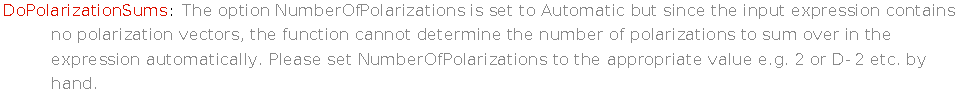
\includegraphics[width=0.6\linewidth]{img/18de6vblvu214.pdf}
\end{figure}

\begin{dmath*}\breakingcomma
\text{\$Aborted}
\end{dmath*}

Here additional user input is needed

\begin{Shaded}
\begin{Highlighting}[]
\NormalTok{DoPolarizationSums}\OperatorTok{[}\NormalTok{xyz}\OperatorTok{,} \FunctionTok{p}\OperatorTok{,}\NormalTok{ NumberOfPolarizations }\OtherTok{{-}\textgreater{}} \DecValTok{2}\OperatorTok{]}
\end{Highlighting}
\end{Shaded}

\begin{dmath*}\breakingcomma
\text{DoPolarizationSums: The input expression contains terms free of polarization vectors. Those will be multiplied with the number of polarizations given by }2.
\end{dmath*}

\begin{dmath*}\breakingcomma
2 \;\text{xyz}
\end{dmath*}
\end{document}
